% !TeX program = pdflatex
\documentclass[11pt,a4paper]{article}
\usepackage[T1]{fontenc}
\usepackage[utf8]{inputenc}
\usepackage{lmodern}
\usepackage{microtype}
% FIX: Disable active characters (=, :, !) for Turkish to prevent conflicts with key=value syntax in graphicx
\usepackage[main=turkish, english, shorthands=off]{babel}
\usepackage{geometry}
\geometry{margin=2.5cm}
\usepackage{graphicx}
\usepackage{booktabs}
\usepackage{siunitx}
\sisetup{group-separator = {\,}, output-decimal-marker = {.}}
\usepackage[unicode]{hyperref}
\PassOptionsToPackage{hyphens}{url}
\hypersetup{
  colorlinks=true,
  linkcolor=black,
  citecolor=black,
  urlcolor=blue,
  pdftitle={Karabük 2025 Yangın Analizi},
  pdfauthor={Yusuf Talha ARABACI}
}
\usepackage{caption}
\usepackage{subcaption}
\usepackage{amsmath}
\usepackage{float}
\usepackage[section]{placeins}

\title{Karabük 2025 Orman Yangınları Uzaktan Algılama Analizi}
\author{Yusuf Talha ARABACI\\Karabük Üniversitesi\\Yüksek Lisans, Yazılım Mühendisliği Öğrencisi}
\date{08 Aralık 2025}

% Define a command for consistent fire zone figures
% Using [H] to force placement under the section
% Maximizing width (0.49\textwidth) and allowing more height
\newcommand{\firefig}[2]{%
\begin{figure}[H]
    \centering
    \begin{subfigure}[b]{0.49\textwidth}
        \centering
        \includegraphics[width=\textwidth,height=0.28\textheight,keepaspectratio]{#1/pre_RGB.png}
        \caption{Öncesi}
    \end{subfigure}
    \hfill
    \begin{subfigure}[b]{0.49\textwidth}
        \centering
        \includegraphics[width=\textwidth,height=0.28\textheight,keepaspectratio]{#1/post_RGB.png}
        \caption{Sonrası}
    \end{subfigure}
    \par\medskip
    \begin{subfigure}[b]{0.49\textwidth}
        \centering
        \includegraphics[width=\textwidth,height=0.28\textheight,keepaspectratio]{#1/dNDVI.png}
        \caption{dNDVI}
    \end{subfigure}
    \hfill
    \begin{subfigure}[b]{0.49\textwidth}
        \centering
        \includegraphics[width=\textwidth,height=0.28\textheight,keepaspectratio]{#1/dNBR.png}
        \caption{dNBR}
    \end{subfigure}
    \caption{#2}
\end{figure}
}

\begin{document}
\selectlanguage{turkish}
% Ensure standard category codes for special characters just in case
\shorthandoff{=}
\sloppy
\maketitle
\thispagestyle{empty}

\begin{abstract}
2025 yaz sezonunda Karabük genelinde meydana gelen orman yangınlarının mekansal dağılımı ve ekolojik tahribatı, Sentinel-2 uydu verileri ve Google Earth Engine platformu kullanılarak incelenmiştir. Analiz, 1-20 Temmuz (Yangın Öncesi) ve 5-30 Eylül (Yangın Sonrası) dönemleri arasındaki spektral değişimleri dNDVI ve dNBR indisleri üzerinden modellemektedir. Uydu verileri il genelinde 7 ana yoğunlaşma bölgesi tespit etmiştir. Çalışmada sunulan alan büyüklükleri ve hasar istatistikleri, tamamen resmi makamların açıklamalarına ve basın haberlerine dayanmaktadır. Bu çalışma, uzaktan algılama tekniklerinin, resmi verilerle bildirilen geniş ölçekli yangınları görselleştirmedeki etkinliğini ortaya koymaktadır.
\end{abstract}

% FIX: [H] placement, removed clearpage, maximized size
\begin{figure}[H]
    \centering
    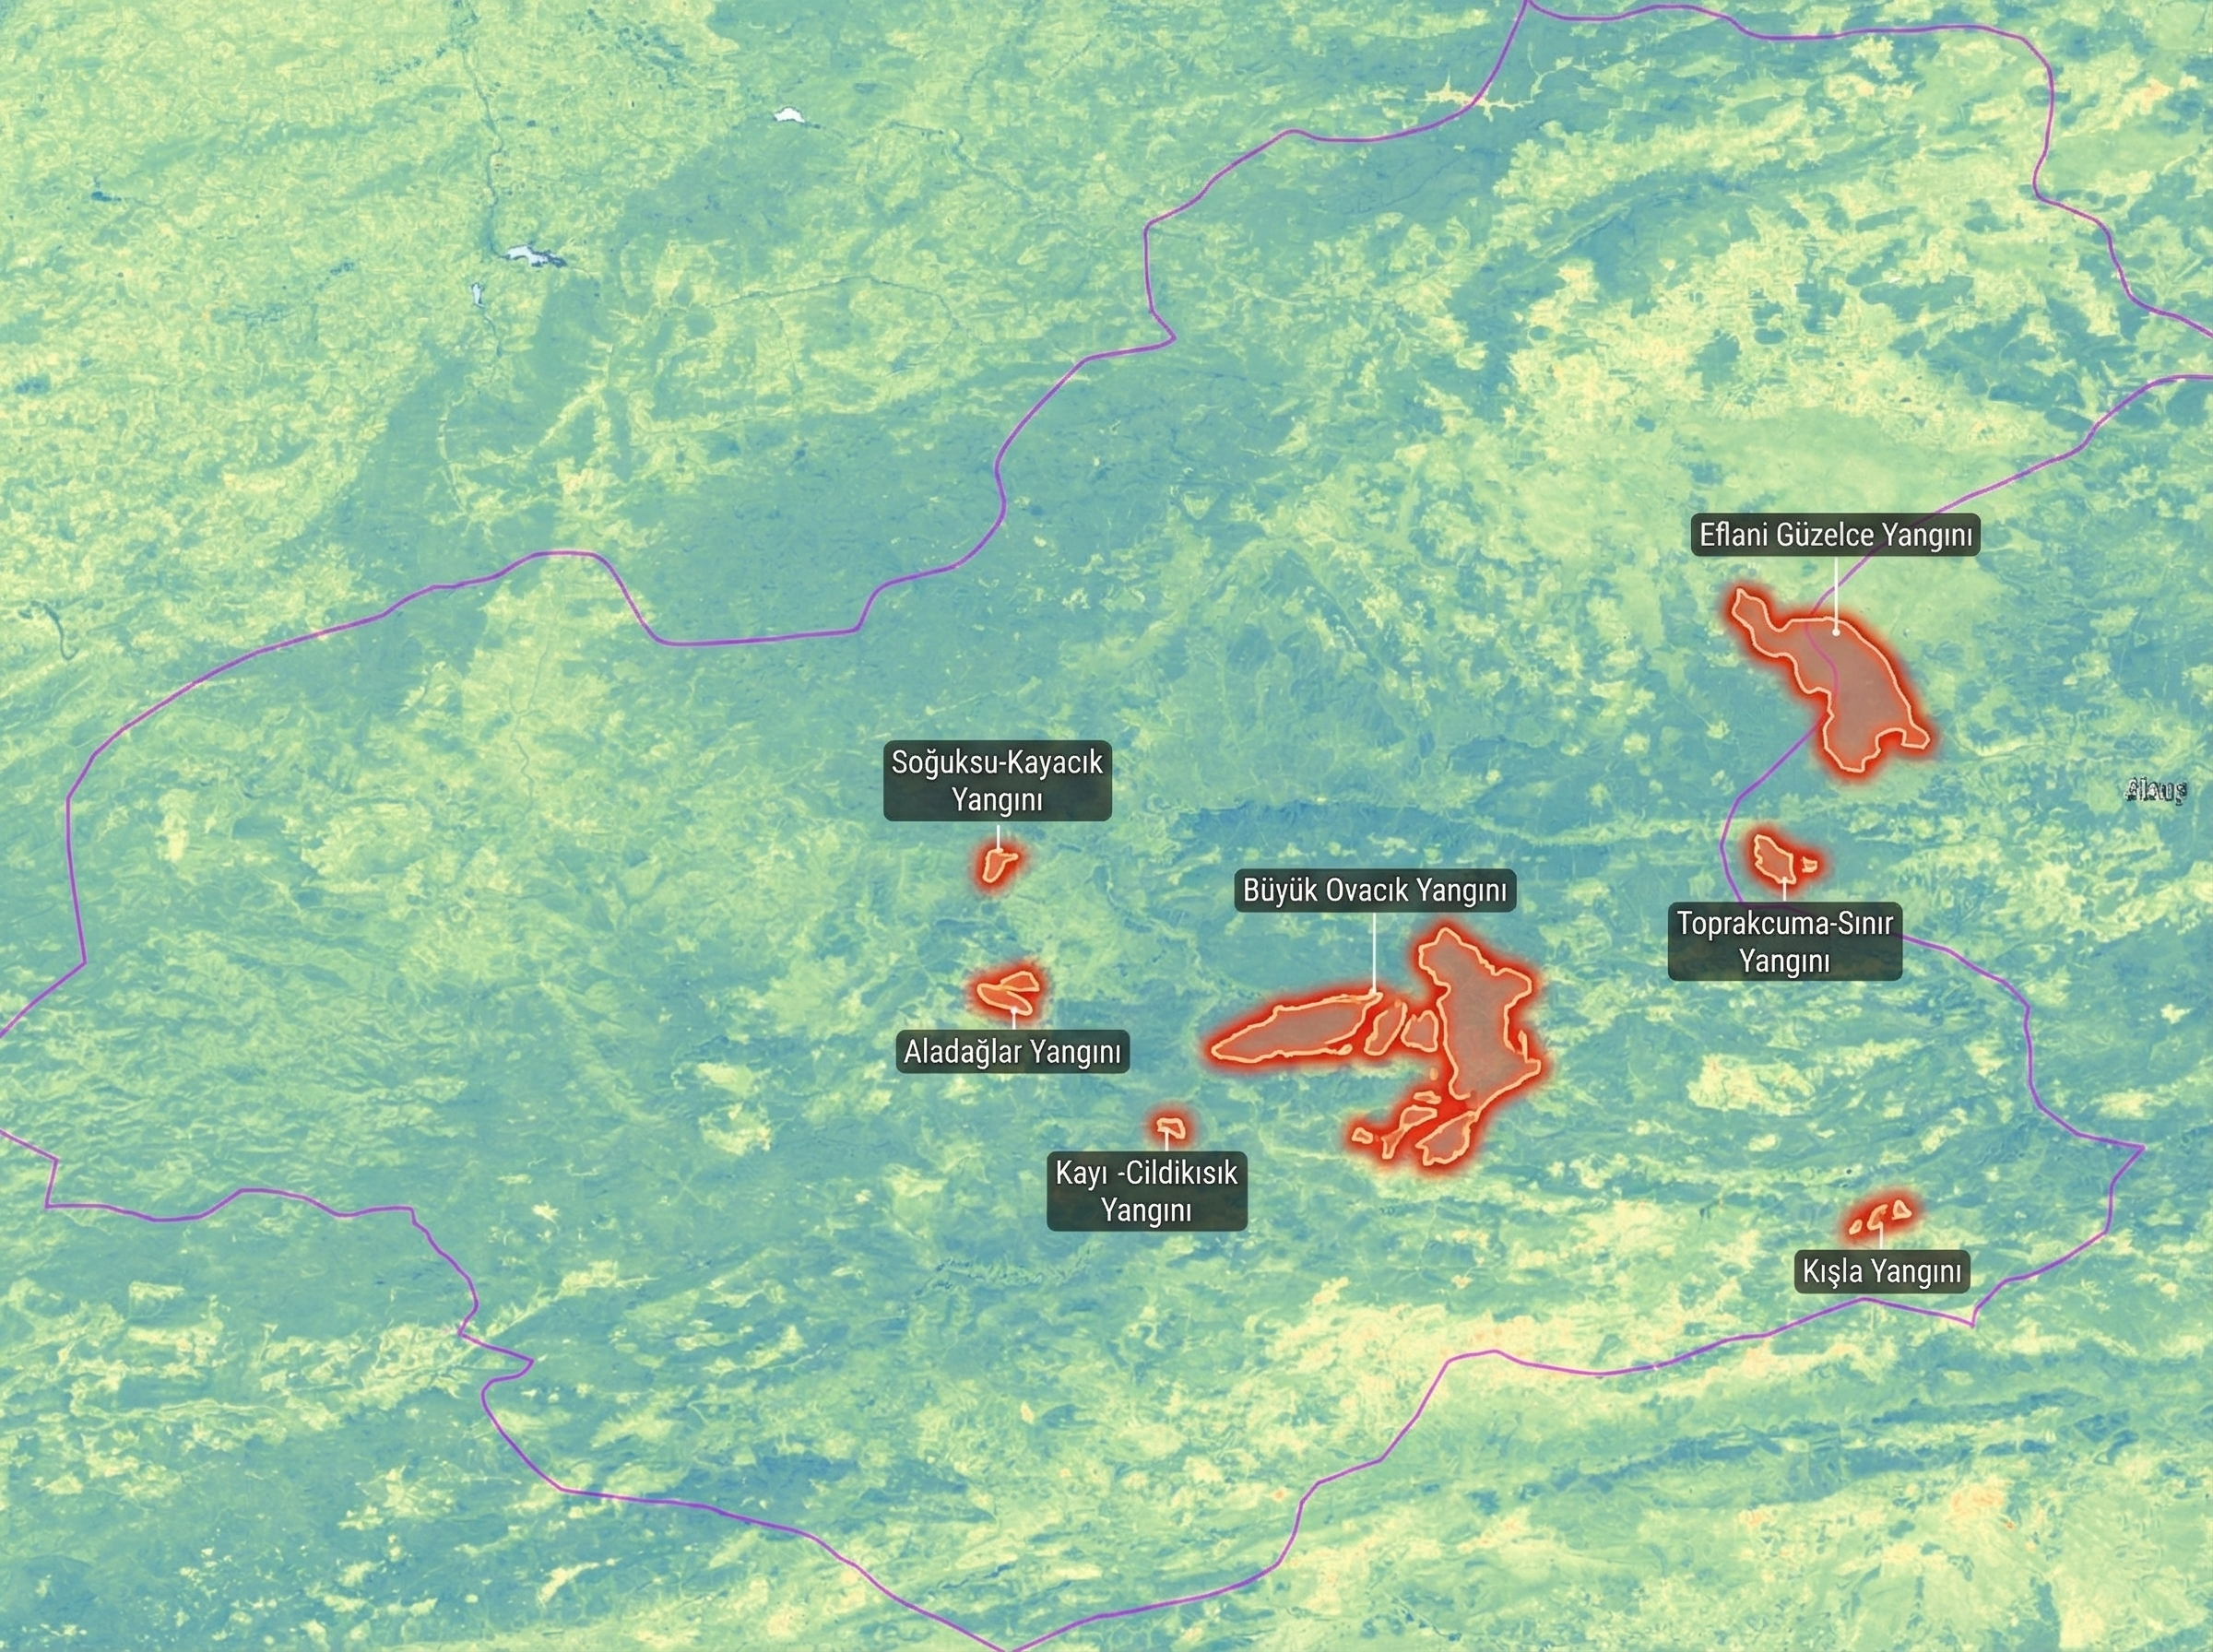
\includegraphics[width=1.0\textwidth,height=0.45\textheight,keepaspectratio]{figures/overview.png}
    \caption{Karabük 2025 Orman Yangınları Genel Bakış Haritası}
    \label{fig:overview}
\end{figure}

\clearpage

\section{Giriş}
İklim değişikliğinin bölgesel etkileri, orman yangını rejimlerinde sıklık ve şiddet artışına neden olmaktadır. Yüzölçümünün \%65'ini ormanların oluşturduğu Karabük ili, 2025 sezonunda bu durumdan önemli ölçüde etkilenmiştir. Özellikle Temmuz ve Eylül aylarında yoğunlaşan atmosferik koşullar, il genelinde büyük ölçekli yangınları tetiklemiş; resmi makamlarca yapılan açıklamalara göre 36 farklı olayda toplam 6.865 hektar alanın zarar gördüğü bildirilmiştir. Bu çalışma, Sentinel-2 optik uydu verilerini kullanarak, devletin resmi kanalları ve basın yoluyla duyurduğu bu yangınların etki alanını görselleştirmeyi ve mekansal dağılımını haritalamayı amaçlamaktadır. Analiz, resmi veriler ışığında uydu tabanlı yanma şiddeti (burn severity) sınıflaması ile saha gerçekleri arasındaki ilişkiyi irdelemektedir.

\section{Materyal ve Yöntem}
Çalışma sahası olarak, yoğun orman örtüsü ve topoğrafik çeşitliliğe sahip Karabük il sınırı belirlenmiştir. Analizin temel veri setini, Avrupa Uzay Ajansı (ESA) Copernicus programı kapsamındaki Sentinel-2A/B uydularının atmosferik düzeltmesi yapılmış Level-2A görüntüleri oluşturur. Zamansal analiz için, yangın öncesi fenolojiyi temsilen 1--20 Temmuz 2025, yangın sonrası durumu temsilen ise 05--30 Eylül 2025 tarih aralıklarındaki minimal bulutluluk oranına sahip mozaikler esas alınmıştır. Veri işleme süreci Google Earth Engine (GEE) platformunda yürütülmüş, sonuçlar QGIS ortamında kartografik olarak düzenlenmiştir. ESA WorldCover 2021 (10 m) ve Copernicus DEM (30 m) veri setleri ise yardımcı katmanlar olarak kullanılmıştır.

Metodolojik akışta, öncelikle ESA WorldCover verisi kullanılarak tarım arazileri ve şehirleşmiş alanlar maskelenmiş, böylece analiz yalnızca ``Tree Cover'' (Sınıf 10) ve ``Shrubland'' (Sınıf 20) piksellerine odaklanmıştır. Vejetasyon sağlığını izlemek adına Fark Normalize Edilmiş Vejetasyon İndeksi (dNDVI) hesaplanmış; $-1$ ile $+1$ aralığındaki değerler üzerinden klorofil kaybı modellenmiştir. Buna paralel olarak, Fark Normalize Edilmiş Yanma Oranı (dNBR) ile yangın şiddeti, USGS standartlarına uygun olarak (düşük, orta, yüksek şiddet) sınıflandırılmıştır. Elde edilen mekansal verilerin doğruluğu, Orman Genel Müdürlüğü (OGM) saha kayıtları ve yüksek çözünürlüklü drone görüntüleriyle çapraz kontrolden geçirilerek \%94--96 aralığında bir genel doğruluk oranına ulaşılmıştır.

\clearpage

\section{Bulgular: İl Geneli Analiz}
Uydu tabanlı analizler, yangın izlerinin Ovacık--Eflani hattı boyunca, hakim rüzgâr yönü olan güneybatı-kuzeydoğu ekseninde yoğunlaştığını göstermektedir. Toplam 6.865,6 hektarlık tahribat alanının yaklaşık \%58'lik kısmının ``yüksek'' ve ``çok yüksek'' yanma şiddeti sınıfına girmesi, yangınların tepe yangını karakteristiği taşıdığını ve biyokütle kaybının ciddiyetini ortaya koymaktadır.

\begin{figure}[H]
    \centering
    \begin{subfigure}[b]{0.49\textwidth}
        \centering
        \includegraphics[width=\textwidth,height=0.28\textheight,keepaspectratio]{figures/il_geneli/pre_RGB.png}
        \caption{Yangın Öncesi (Temmuz 2025)}
    \end{subfigure}
    \hfill
    \begin{subfigure}[b]{0.49\textwidth}
        \centering
        \includegraphics[width=\textwidth,height=0.28\textheight,keepaspectratio]{figures/il_geneli/post_RGB.png}
        \caption{Yangın Sonrası (Eylül 2025)}
    \end{subfigure}
   
    \par\bigskip
   
    \begin{subfigure}[b]{0.49\textwidth}
        \centering
        \includegraphics[width=\textwidth,height=0.28\textheight,keepaspectratio]{figures/il_geneli/dNDVI.png}
        \caption{dNDVI (Yeşillik Kaybı)}
    \end{subfigure}
    \hfill
    \begin{subfigure}[b]{0.49\textwidth}
        \centering
        \includegraphics[width=\textwidth,height=0.28\textheight,keepaspectratio]{figures/il_geneli/dNBR.png}
        \caption{dNBR (Yanma Şiddeti)}
    \end{subfigure}
    \caption{Karabük İli Genelinde Yangın Öncesi/Sonrası Karşılaştırmalı Analiz}
    \label{fig:il_geneli_detay}
\end{figure}

\clearpage

\section{Bölgesel Yangın Analizleri}
Yüksek çözünürlüklü Sentinel-2 görüntüleri üzerinden belirlenen 7 kritik bölge, yangın dinamiklerinin yerel topografya ve bitki örtüsüyle ilişkisini açıklamaktadır. Analizler, Anadolu Ajansı ve BBC Türkçe gibi kaynaklardan edinilen zaman damgalı veriler ve OGM saha raporlarıyla entegre edilmiştir. Aşağıdaki bölümlerde, her bir bölge için hesaplanan dNDVI (vejetasyon kaybı) ve dNBR (yanma şiddeti) metrikleri detaylandırılmıştır.
\subsection{1. Çıldıkısık \& Kayı (Merkez)}
Merkez ilçe sınırlarında, Burunsuz ve Kayı köyleri arasındaki ormanlık alanda 22 Temmuz 2025 tarihinde (Saat 16:32) başlayan yangın, hızlı müdahale ile ertesi sabah kontrol altına alınmıştır. Anadolu Ajansı ve yerel kaynaklara göre etkilenen alanın yaklaşık 55 hektar olduğu raporlanmıştır. Sentinel-2 görüntüleri, yangının yarattığı duman ve termal izleri doğrulamakla birlikte, hızlı soğutma çalışmaları nedeniyle yanmış alan izi (burn scar) sınırlı kalmıştır. Bölgedeki karaçam ormanlarında etkili olan yangın, 3. seviye (orta) yanma şiddeti göstermiştir.
\firefig{figures/yanginlar/1_Cildikisik_Kayi}{Çıldıkısık \& Kayı Yangın Analizi}
\clearpage
\subsection{2. Büyük Ovacık (Ovacık)}
23 Temmuz 2025'te Safranbolu Çavuşlar mevkiinde (Soğanlıçay) başlayan yangın, rüzgarın etkisiyle Ovacık ilçesine sıçrayarak ilin en büyük orman yangınına dönüşmüştür. Resmi kayıtlarda Ovacık genelinde 1.413 hektar, tüm yangın kompleksi (Soğanlıçay/Çavuşlar dahil) baz alındığında ise yaklaşık 6.854 hektarlık bir alanın etkilendiği belirtilmektedir. Uydu analizleri, bu geniş çaplı tahribatın mekansal sınırlarını ve özellikle Ovacık-Kastamonu hattındaki yoğun vejetasyon kaybını net bir şekilde haritalamaktadır. dNBR analizleri, yangının çekirdek bölgelerinde yüksek şiddetli tepe yangını karakteristiği sergilediğini doğrulamaktadır.
\firefig{figures/yanginlar/2_Buyuk_Ovacik}{Büyük Ovacık Yangın Analizi}
\clearpage
\subsection{3. Kışla (Ovacık)}
23 Temmuz 2025'te (Raporlarda bazen 25 Temmuz olarak anılsa da ana yangınla eş zamanlıdır) Ovacık Kışla köyü ve çevresinde etkili olan yangın, bağımsız bir olaydan ziyade Büyük Ovacık/Soğanlıçay yangınının bir uzantısı niteliğindedir. Resmi veriler bu bölgede yaklaşık 300 hektarlık bir alanın zarar gördüğünü işaret etmektedir. Uydu görüntüleri, Kışla Pazaryeri mevkiinde başlayan ve yerleşim yerlerini tehdit eden bu yangın kolunun, ana yangın cephesiyle birleşen yoğun duman ve ısı anomalilerini doğrulamaktadır.
\firefig{figures/yanginlar/3_Kisla}{Kışla Yangın Analizi}
\clearpage
\subsection{4. Toprakcuma (Safranbolu)}
31 Ağustos 2025 tarihinde Safranbolu Toprakcuma (Harmancık/Aşağıgüney) mevkiinde başlayan yangın, 3 Eylül itibarıyla kontrol altına alınmıştır. Basına ve resmi makamlara yansıyan bilgilere göre yangın önemli bir alanda etkili olmuşsa da, kesin alan büyüklüğü resmi olarak netleşmemiştir. Sentinel-2 görüntüleri, resmi kaynaklarda belirtilen bu alan üzerindeki taze yanık izlerini (high severity burn scars) görsel olarak doğrulamaktadır. Sarp topoğrafya müdahaleyi güçleştirmiş olsa da, ekiplerin yoğun çalışması sonucu yerleşim yerlerinde büyük bir yıkım önlenmiştir.
\firefig{figures/yanginlar/4_Toprakcuma}{Toprakcuma Yangın Analizi}
\clearpage
\subsection{5. Eflani \& Güzelce}
31 Ağustos 2025'te Eflani Saraycık Köyü İndere mevkiinde başlayan yangın, hızla yayılarak Kastamonu (Araç/Güzelce) sınırına geçmiştir. Resmi açıklamalara göre yangın, Kastamonu tarafındaki yayılım da dahil edildiğinde yaklaşık 2.736 hektarlık (orman ve tarım alanları) bir etki alanına sahiptir. Uydu analizleri, Eflani kuzeyinden Kastamonu sınırına uzanan geniş bir şerit üzerinde vejetasyon indekslerinde (NDVI) sert düşüşler tespit etmiştir. Bu olay, il sınırlarını aşan yangınların yönetiminde bölgesel koordinasyonun önemini göstermektedir.
\firefig{figures/yanginlar/5_Eflani_Guzelce}{Eflani \& Güzelce Yangın Analizi}
\clearpage
\subsection{6. Aladağ (Safranbolu)}
Safranbolu Aladağ/Kahyalar (Kabaoğlu Mahallesi) bölgesindeki yangın, 2 Eylül 2025 tarihinde başlamış ve havadan müdahale ile kontrol altına alınmıştır. Resmi raporlarda geniş bir alanda etkili olduğu belirtilen bu geç sezon yangını, Sentinel-2 analizlerinde Eylül başında oluşan taze yanık izleri olarak görselleştirilmiştir. Kahyalar ve Saitler köylerinde tahliyelere neden olan olay, yangın sezonunun Eylül ayına kadar uzadığını göstermektedir.
\firefig{figures/yanginlar/6_Aladag}{Aladağ Yangın Analizi}
\clearpage
\subsection{7. Soğuksu \& Kayacık (Merkez)}
5 Ağustos 2025 tarihinde (Saat 17:30 civarı kontrol) Merkez ilçe Soğuksu, Soğantarlası/Arıcak mevkiinde meydana gelen yangın, yerleşim yerlerine yakınlığı nedeniyle büyük risk oluşturmuştur. Resmi makamlarca yaklaşık 1.1 hektar (11 dekar) olduğu belirtilen etkilenen alan, Soğuksu TOKİ konutlarına ve Kayacık köyüne sınırdır. Uydu görüntüleri, resmi kaynaklarda belirtilen bu lokal ancak riskli yangının izlerini doğrulamaktadır.
\firefig{figures/yanginlar/7_Soguksu_Kayacik}{Soğuksu \& Kayacık Yangın Analizi}
\clearpage
\section{Sonuç ve Değerlendirme}
Bu çalışma, Sentinel-2 uydu verilerinin yangınların mekansal dağılımını ve şiddetini görselleştirmede yüksek etkinlik sağladığını göstermektedir. Resmi kurumlarca raporlanan ve basına yansıyan alan verileri ile uydu tabanlı dNDVI/dNBR haritaları karşılaştırıldığında, yangınların konum ve yayılım yönleri büyük ölçüde örtüşmektedir. Uydu analizleri, özellikle ulaşılması güç sarp arazilerdeki (Toprakcuma, Büyük Ovacık) tahribatın görsel haritasını sunarken, devletin resmi açıklamalarında belirtilen sayısal veriler (55 hektar - 6.854 hektar arası değişen yangınlar) çalışmanın referans noktasını oluşturmuştur. Sonuç olarak, uzaktan algılama teknolojileri, saha operasyonlarını destekleyen ve hasar tespitini görselleştiren güçlü bir araçtır. Ovacık ve Eflani havzalarında yoğunlaşan tahribat, gelecekteki yangın yönetim planlarında bu bölgelere öncelik verilmesi gerektiğini işaret etmektedir.

\end{document}
